\documentclass[journal,12pt,twocolumn]{IEEEtran}
\IEEEoverridecommandlockouts
\usepackage{cite}
\usepackage{amsmath,amssymb,amsfonts,bm}
\usepackage{mathtools}
\usepackage{tkz-euclide} 
\usetikzlibrary{calc,math}
 \usepackage{caption}
\usepackage{listings}
\usetkzobj{all}
\let\vec\mathbf
\newcommand{\myvec}[1]{\ensuremath{\begin{pmatrix}#1\end{pmatrix}}}
\newcommand{\norm}[1]{\left\lVert#1\right\rVert}


\begin{document}

\title{Assignment 3}

\author{\IEEEauthorblockN{Pulkit Saxena}}
\maketitle
\section{Question 1.36 Geolin.pdf }
BE and CF are two equal altitudes of a triangle ABC. Using RHS congruence rule, prove that the triangle ABC is isosceles.
\section{Solution}

BE and CF are two equal altitudes of a triangle ABC.
\captionsetup{justification=centering}

\begin{figure}[!h]
\centering
\resizebox{.5\columnwidth}{!}
{
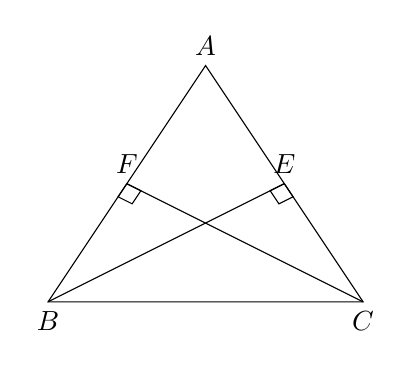
\begin{tikzpicture} 
        \coordinate (A) at (2, 3) {};
        \coordinate (B) at (0, 0) {};
        \coordinate (C) at (4, 0) {};
        \coordinate (F) at (1, 1.5) {};
        \coordinate (E) at (3, 1.5) {};
\draw (A)node[above]{$A$}--(B)node[below]{$B$}--(C)node[below]{$C$}--cycle;
\draw (B)node[below]{}--(E)node[above]{$E$};
\draw (C)node[below]{}--(F)node[above]{$F$};
\tkzMarkRightAngle[size=.2](B,E,C);
\tkzLabelAngle[dist=.5](B,E,C){};
\tkzMarkRightAngle[size=.2](C,F,B);
\tkzLabelAngle[dist=.5](C,F,B){};
\end{tikzpicture}
}
\caption{Triangle with equal altitudes on two sides}
\label{myfig}
\end{figure}
Given:-\\
1) Altitudes are Equal means their magnitude are same
 \begin{align}
 	\norm{\vec{E - B}} = \norm{\vec{F - C}} \label{1}
 \end{align}
2) Altitude makes right angle at the base therefore $\cos 90 =0$ therefore  FC $\perp$ BF and EB $\perp$ CE where $\textbf{m}$ is the directional vectors.
\begin{align}
\textbf{m}_{FC} \textbf{m}_{BF} = 0 \label{2}\\
\textbf{m}_{EB} \textbf{m}_{CE} = 0 \label{3}
\end{align}

From equation {\ref{2}}
\begin{align}
    \myvec{B-F}\myvec{F-C}^T=0 && \myvec{F-C}\myvec{B-F}^T=0\label{4}
\end{align}
From equation {\ref{2}} and using equation {\ref{4}} 
\begin{align}
    \myvec{B-C}\myvec{B-C}^T\\
    =\myvec{B-F+F-C}\myvec{B-F+F-C}^T
    \end{align}
    \begin{align}
      =\myvec{B-F}\myvec{B-F}^T+\myvec{F-C}\myvec{F-C}^T 
    \end{align}
\begin{align}
   \norm{B-C}^2=\norm{B-F}^2+\norm{F-C}^2\label{8} 
    \end{align}
    Similarly\\
    From Equation {\ref{3}}
    \begin{align}
        \myvec{E-B}\myvec{E-C}^T=0 && \myvec{E-C}\myvec{B-E}^T=0\label{9}
        \end{align}
From equation {\ref{3}} and using equation {\ref{9}}  
\begin{align}
    \myvec{B-C}\myvec{B-C}^T\\
    =\myvec{B-E+E-C}\myvec{B-E+E-C}^T
    \end{align}
    \begin{align}
      =\myvec{B-E}\myvec{B-E}^T+\myvec{E-C}\myvec{E-C}^T 
    \end{align}
\begin{align}
   \norm{B-C}^2=\norm{B-E}^2+\norm{E-C}^2\label{13}
    \end{align}        
    Equating Equation \ref{8} and equation \ref{13} and using equation \ref{1}
    \begin{align}
      \norm{B-F}^2+\norm{F-C}^2 = \norm{B-E}^2+\norm{E-C}^2  
    \end{align}
    \begin{align}
       \norm{B-F}^2=\norm{E-C}^2\\
       =\norm{B-F}=\norm{E-C}\label{16}
    \end{align}
    
    Let $\angle FBC=\theta_1$  and  $\angle EBC=\theta_2$
    \begin{align}
        \myvec{B-F}\myvec{B-C}^T=\norm{B-F}\norm{B-C}\cos\theta_1\\
        \cos{\theta_1}=\frac{\myvec{B-F}\myvec{B-C}^T}{\norm{B-F}\norm{B-C}}\\
        \cos{\theta_1}=\frac{\myvec{B-F}\myvec{B-F+F-C}^T}{\norm{B-F}\norm{B-C}}\\
        \cos{\theta_1}=\frac{\myvec{B-F}\myvec{B-F}^T +\myvec{B-F}\myvec{F-C}^T}{\norm{B-F}\norm{B-C}}
        \end{align}
        From Equation {\ref{4}}
        \begin{align}
          \cos{\theta_1}=\frac{\myvec{B-F}\myvec{B-F}^T}{\norm{B-F}\norm{B-C}} \\
          \cos{\theta_1}=\frac{\norm{B-F}^2}{\norm{B-F}\norm{B-C}}\\
          \cos{\theta_1}=\frac{\norm{B-F}}{\norm{B-C}}
        \end{align}
        Similarly for $\angle EBC=\theta_2$
        \begin{align}
        \myvec{C-E}\myvec{B-C}^T=\norm{C-E}\norm{B-C}\cos\theta_2\\
        \cos{\theta_2}=\frac{\myvec{C-E}\myvec{B-C}^T}{\norm{C-E}\norm{B-C}}\\
        \cos{\theta_2}=\frac{\myvec{C-E}\myvec{B-E+E-C}^T}{\norm{C-E}\norm{B-C}}\\
        \cos{\theta_2}=\frac{\myvec{C-E}\myvec{B-E}^T +\myvec{C-E}\myvec{E-C}^T}{\norm{C-E}\norm{B-C}}
        \end{align}
        From Equation {\ref{9}}
        \begin{align}
          \cos{\theta_2}=\frac{\myvec{C-E}\myvec{C-E}^T}{\norm{C-E}\norm{B-C}} \\
          \cos{\theta_2}=\frac{\norm{C-E}^2}{\norm{C-E}\norm{B-C}}\\
          \cos{\theta_2}=\frac{\norm{C-E}}{\norm{B-C}}
        \end{align}
        From equation \ref{16} we know $\norm{B-F}=\norm{E-C}$ we conclude
        \begin{align}
            \cos\theta_1=\cos\theta_2
            \implies\theta_1=\theta_2
        \end{align}
        So the sides opposite to equal angles are equal. Hence AB=AC hence the given Triangle is isosceles.
    \end{document}


